\section{Introduction}
\label{sec:introduction}

Medical AI is still commonly evaluated as a static predictor: an image, waveform, pathology slide, note, or structured record is mapped to a label, risk score, report, or triage decision. Clinical decisions pose a different problem. An oncologist choosing among chemotherapy, radiotherapy, surgery, and surveillance needs to reason about how the same patient's state may evolve after an action that could actually be taken. Comparable questions arise in sepsis management, longitudinal monitoring, image acquisition, surgery, and physiological control. The shift from prediction to world modeling is therefore not defined by adopting a particular architecture. It is a shift from asking what is present, or what usually follows, to asking how a patient or clinical environment changes and whether those changes can inform action.

Several literatures now approach this problem under overlapping names. Recent reviews connect medical state representation, future prediction, intervention-conditioned simulation, and planning \citep{Qazi2025BeyondGenerativeAI,Saeed2026MedicalWorldModel,Liu2026MedicalWorldModelsReview,Wang2026TowardsBiomedicalWorldModels}. Digital twins emphasize patient-specific virtual counterparts and repeated updating \citep{Iqbal2025consensusstatementon,Katsoulakis2024Digitaltwinshealth,Ghatti2023DigitalTwinsHealthcare}. Patient-trajectory and EHR foundation models learn longitudinal event distributions \citep{Kraljevi_2024Foresightgenerativepretrained,Waxler2025GenerativeMedicalEvent,Guo2026Systematicreviewfoundation}. Treatment-aware simulators, model-based clinical reinforcement learning, and embodied medical systems place actions more explicitly inside the modeled process \citep{Yang2025MedicalWorldModel,Ding2025CLARITYMedicalWorld,Raghu2018ModelBasedReinforcement,Chen2026ECGWMPhysiology,Sivakumar2026SWoMoNeuroSymbolic}. These lineages share an interest in dynamics, yet they do not make the same scientific claim.

The resulting terminology is difficult to interpret. A representation model may be called a world-model backbone although it has no directed temporal transition. A future-image generator may capture temporal change but expose no clinical action. A treatment-conditioned generator may allow an intervention label to be changed while learning only associations in retrospective care. A planner may optimize actions through a learned simulator even when that simulator does not identify patient-specific treatment effects. Treating all four systems as equivalent obscures both what has been achieved and what remains unsupported.

This survey addresses that ambiguity through a claim-to-evidence view of medical world models. We ask three questions. First, what form of capability is actually implemented: state representation, future prediction, action-conditioned simulation, counterfactual outcome reasoning, or model-based planning and control? Second, in which clinical applications and data regimes has that capability been studied? Third, does the available evidence support the state, action, transition, outcome, and validation commitments required by the claim? Figure~\ref{fig:roadmap} gives the conceptual reading map. Capability supplies the main axis; application, architecture, and modality describe where and how a capability is realized; the SATO-V contract evaluates how far the supporting evidence extends.

\begin{figure}[t]
\centering
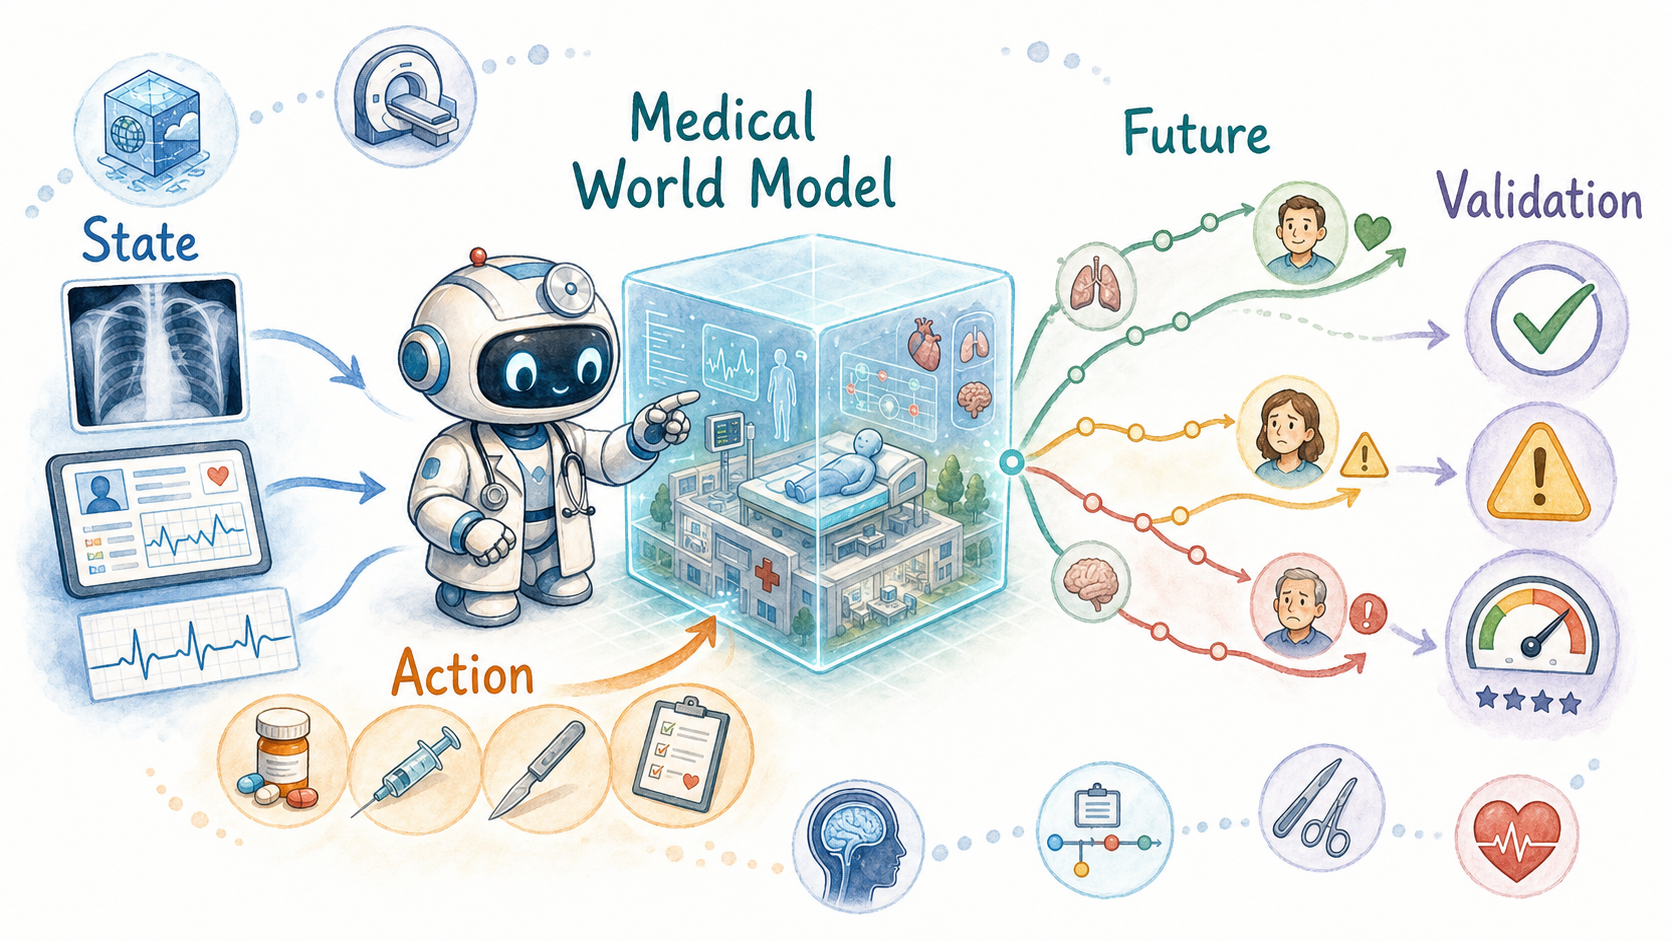
\includegraphics[width=\linewidth]{figures/fig_roadmap_imagegen_v3.png}
\caption{A visual definition of a medical world model. Patient state evidence and executable clinical actions enter a simulator-like model of the medical environment; the model rolls forward plausible future trajectories and exposes outcome or validation targets. The small visual badges indicate the paper families reviewed later in the article, including imaging, EHR trajectories, causal treatment modeling, surgical simulation, physiological signals, and general world-model backbones.}
\label{fig:roadmap}
\end{figure}


Our central standard is \emph{clinical-action validity}. A clinically meaningful state must be linked to an action that can be chosen or executed; the modeled transition must respond to that action; the resulting outcome must match the decision being invoked; and validation must address the relevant horizon and use. This standard is stricter than visual realism or trajectory plausibility. A generated future MRI can be useful for interpolation, prognosis, or education without supporting treatment selection. Conversely, an acquisition or surgical simulator may have unusually clear actions even when its patient-outcome evidence remains limited. Clinical-action validity is therefore not a binary badge. It is a way to state precisely which part of a decision claim is supported and which part is not.

Three recurrent gaps motivate this approach. The first concerns action semantics. Time, disease stage, a medication observed in the record, a desired output label, and an executable intervention play different roles, even though each may enter a model as a token or conditioning variable. The second concerns the distinction between observed and alternative outcomes. Conditioning on treatment does not by itself establish what would have happened to the same patient under another treatment. The third concerns validation. A rollout can be realistic on held-out retrospective data yet unreliable under a new policy, at a longer horizon, or for actions weakly represented in the training distribution. These gaps are not ancillary limitations; they determine the strongest defensible interpretation of a system.

The review is organized around five non-cumulative capability levels. The ordering follows the questions posed by a model, not a claim that every system should climb a single maturity ladder. Level~1 constructs a clinically meaningful state but does not model a directed future. Level~2 predicts what is likely to happen next without exposing a settable action. Level~3 simulates a future after an explicit action, while remaining agnostic about whether observational conditioning identifies a causal effect. Level~4 estimates outcomes under alternatives for the same patient or state under an explicit causal or structural contract. Level~5 uses a learned or mechanistic model to rank, optimize, or control actions. A Level~5 planner need not satisfy Level~4 counterfactual identification, and a Level~4 estimator need not implement a planner. This separation is essential in medicine, where computational capability and evidential validity frequently advance at different rates.

\paragraph{Contributions.} This survey makes four contributions. First, it provides an operational definition of medical world modeling centered on state transition and clinical-action validity. Second, it adapts prior capability ladders into five non-cumulative task contracts with explicit adjacent boundaries, giving particular attention to the transition from forecasting to action-conditioned simulation and from conditioning to counterfactual estimation. Third, it synthesizes the literature within each capability level across clinical applications and representative model designs, while using SATO-V to distinguish implemented form from evidential support. Fourth, it derives a cross-level assessment and research agenda focused on action semantics, causal identification, decision-aligned validation, external generalization, and reporting standards. The aim is not to claim ownership of the underlying progression, which has clear precedents, but to make its medical evidence boundaries useful for reading and evaluating the field.

\paragraph{Organization.} Section~\ref{sec:background} places this review relative to general world models, causal reasoning, digital twins, patient-trajectory modeling, and recent medical surveys. Section~\ref{sec:framework} defines the existence boundary, SATO-V contract, capability levels, and secondary analytical lenses. Sections~\ref{sec:level1}--\ref{sec:level5} form the core of the survey. Each begins with the minimum capability contract, examines the clinical evidence and representative designs that instantiate it, evaluates characteristic failure modes, and closes with the evidence needed to cross the next boundary. Section~\ref{sec:synthesis} then compares capabilities across applications, architectures, and SATO-V evidence without reintroducing a competing taxonomy. Section~\ref{sec:agenda} turns the recurring gaps into a research agenda and states the limitations of the review. Detailed search, coding, and boundary protocols are provided in the appendices.
